Test Case~1c repeats the exercise from Case~1a, with the difference that the discrete fragility function specifies a minimum ground motion intensity, below which the probability of exceedance for all damage states is assumed to be zero.

\begin{table}[htbp]

\centering
\begin{tabular}{ l c c l }

\hline
\rowcolor{anti-flashwhite}
\bf{GMF \#} & \bf{Site} & \bf{PGA (g)}\\
\hline
1 & 1 & 1.300 \\
2 & 1 & 0.044 \\
3 & 1 & 0.220 \\
4 & 1 & 1.000 \\
5 & 1 & 1.200 \\
\hline
\end{tabular}

\caption{Five precomputed ground motion fields at a single site}
\label{tab:gmfs-diff-l1-5b}
\end{table}

Table~\ref{tab:gmfs-diff-l1-5b} lists the five ground motion values used in this test case, and Table~\ref{tab:ff-disc-tax1-zndl} the discrete fragility function used in this test case. The "no damage limit" is specified to be $0.3 g$.  The fragility model is shown in Figure~\ref{fig:ff-disc-tax1-nzndl}.

\begin{figure}[htbp]
\centering
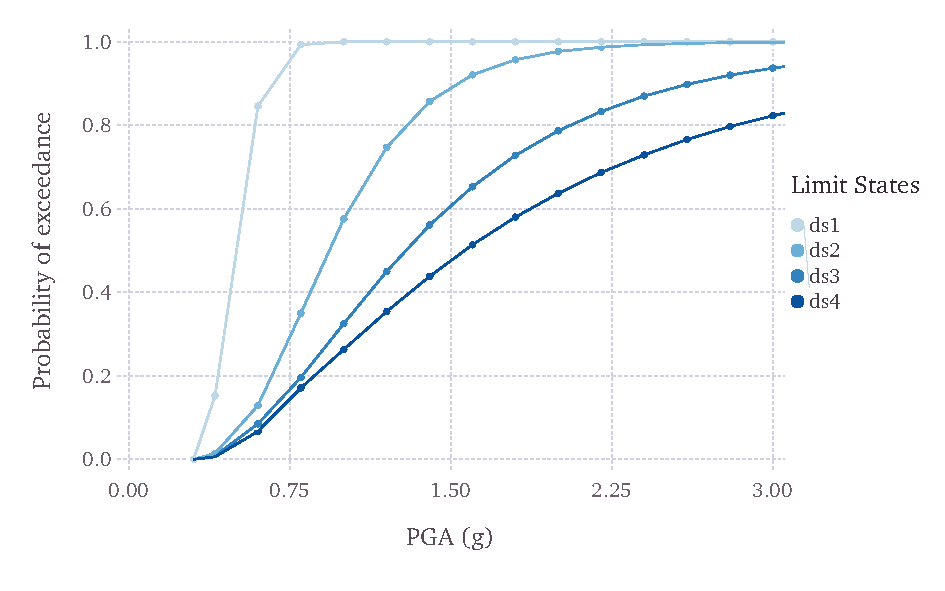
\includegraphics[width=12cm]{qareport/figures/fig-ff-disc-tax1-nzndl}
\caption{Discrete fragility model with four damage states and a nonzero no damage limit}
\label{fig:ff-disc-tax1-nzndl}
\end{figure}

The ground motion values at the location of the single asset are $[1.3, 0.044, 0.22, 1.0, 1.2] g$. The calculation of the damage state exceedance probabilities proceeds in exactly the same manner as demonstrated in Case~1a, except that for the ground motion values of $0.044 g$ and $0.22 g$, the probabilities for all four damage states are assumed to be zero.

We have the following sets of damage state probabilities:

\begin{itemize}
	\item GMF1: $[0.000, 0.198, 0.2965, 0.1095, 0.396]$
	\item GMF2: $[1.000, 0.000, 0.000, 0.000, 0.000]$
	\item GMF3: $[1.000, 0.000, 0.000, 0.000, 0.000]$
	\item GMF4: $[0.000, 0.424, 0.251, 0.062, 0.263]$
	\item GMF5: $[0.000, 0.253, 0.297, 0.096, 0.354]$
\end{itemize}

The mean and standard deviation of the four damage state probabilities and also the probability of observing no damage is now calculated using the above set of probabilities collected from each of the five ground motion simulations.